\documentclass[12pt]{article}
\usepackage[utf8]{inputenc}
\usepackage{amssymb}
\usepackage{makeidx}
\usepackage[english]{babel}
\usepackage{graphicx}
\usepackage{amsfonts,amsmath,amssymb,amsthm}
\usepackage{oldgerm}
\usepackage{mathrsfs}
\usepackage[active]{srcltx}
\usepackage{verbatim}
\usepackage[toc,page]{appendix}
\usepackage{aliascnt}
\usepackage{array}
\usepackage{hyperref}
\usepackage[textwidth=4cm,textsize=footnotesize]{todonotes}
\usepackage{xargs}
\usepackage{cellspace}
\usepackage[Symbolsmallscale]{upgreek}
\usepackage{geometry}
\usepackage{hyperref}
\usepackage{array}
\geometry{top=3.5cm, bottom=3.5cm, left=3.5cm , right=3.5cm}
\usepackage{fancyhdr}
\pagestyle{fancy}

\usepackage{graphicx}
\usepackage{caption}
\usepackage{subcaption}
\graphicspath{{figures/}}
\usepackage{enumerate}
\usepackage{xcolor}
\usepackage{algorithm,algorithmic}  

\newcommand{\x}[2]{x_{#1}^{(#2)}}
\newcommand{\w}[2]{w_{#1}^{(#2)}}
\newcommand{\tw}[2]{\tilde{w}_{#1}^{(#2)}}
\newcommand{\p}[2]{\xi_{#1}^{(#2)}}
\newcommand{\tp}[2]{\tilde{\xi}_{#1}^{(#2)}}
\newcommand{\ta}[2]{\tau_{#1}^{(#2)}}
\newcommand{\rmd}{\mathrm{d}}
\newcommand{\eqsp}{\;}
\newcommand{\1}{\mathrm{1}}
\newcommand{\com}[1]{{\color{gray} // #1}}
\newcommand{\mP}{\mathbb{P}}
\newcommand{\E}{\mathbb{E}}
\newcommand{\qk}{q_{k}}
\newcommand{\acom}[1]{\textit{\color{gray} //#1}}
\newcommand{\Oz}{Z}%Letter for the Ozaki approximation
\newcommand{\Jk}{J_{\alpha}^k}%Command for Jacobian of alpha
\newcommand{\mw}{\mathsf{w}}%For bridge realisations
\newcommand{\U}{\mathsf{U}}
\newcommand{\Lo}{\mathsf{L}}
%\newcommand{\qk}{q^{\Delta t_k}_{\theta}}
\newtheorem{lemma}{Lemma}
\newtheorem{proposition}{Proposition}
\newcommand{\hQ}{\widehat{Q}}
\newcounter{hypA}
\newenvironment{hypA}{\refstepcounter{hypA}\begin{itemize}
\item[{\bf H\arabic{hypA}}]}{\end{itemize}}
%%ENvironmment assumption
\newcounter{defcounter}
\setcounter{defcounter}{0}
\newenvironment{assumpt}{%
\addtocounter{equation}{-1}
\refstepcounter{defcounter}
\renewcommand\theequation{\textbf{A}\thedefcounter}
\usepackage{float}
\begin{equation}}
{\end{equation}}
\begin{document}

\author{Pierre Gloaguen\footnotemark[1] \and Marie-Pierre Etienne\footnotemark[1] \and Sylvain Le {C}orff\footnotemark[2]}
 
\footnotetext[1]{AgroParistech, UMR MIA 518, F-75231 Paris, France.}
\footnotetext[2]{Laboratoire de Math\'ematiques d'Orsay, Univ. Paris-Sud, CNRS, Universit\'e Paris-Saclay.}


\title{Efficient online Sequential Monte Carlo smoother for partially observed stochastic differential equations}

\lhead{Gloaguen et al.}
\rhead{Particle smoother for SDE}

\maketitle

The authors are grateful to the associate editor and the anonymous referees for their comments to improve the manuscript. The paper has been modified to take these remarks into account and also carefully proof read to remove remaining typos and minor mistakes. We provide below detailed answers for all comments.

\subsection*{Referee 1}
{\em I have two major comments that I think should be addressed before publishing. First of all the whole presentation is written as given a  fixed observation record $(Y_k)_{1\le k \le n}$, one of the main points of the PaRIS algorithm, which you rely on, is the ability to work with data streams of observations with a  fixed memory usage. 
Maybe it would be a good idea to include this in the paper.}

\vspace{.3cm}

As pointed by the Referee, one of the best feature of PaRIS algorithm is that it may be implemented "online", processing the observations $(Y_k)_{k\ge 1}$ as they are received, without any storage. This may be seen for instance in steps (i)-(iii) in pages 8-9 which describe the way the intermediate quantities $(\tau_k^i)_{1\le i \le N}$ can be computed at each time step. Each time a new observation $Y_{n+1}$ is received, these quantities can be updated only using $Y_{n+1}$, $(\tau_n^i)_{1\le i \le N}$ and the particle filter at time $n$. This means that storage requirements do not increase. The update is stopped when the last observations is received to compute the approximation of the smoothed additive functional. 

This remark was added after steps (i)-(iii) to highlight the online property of the extension of PaRIS algorithm (with no additional storage requirements). The introduction also insists on this property of the algorithm.

In common applications (for instance in the cas of the EM algorithm),  the smoothed additive functional to be computed is known in advance, this is the reason why we chose to stop the updates for a given arbitrary time $n$, but it is now clear that the algorithm may be stopped at any time.

\vspace{1cm}

{\em Secondly in the algorithm presented on page 9, it says to draw $M$ samples from $\zeta_k$ while not mentioning
what to do with these. This should be specified in the manuscript.}

\vspace{.3cm}

The way the unbiased estimation of $q_k(\xi^{I_k^\ell}_{k-1},\xi^\ell_k)$ was computed was indeed not clear. We only stated the existence of a random variable $\zeta_k$ such that $\widehat{q}_k(\xi^{I_k^\ell}_{k-1},\xi^\ell_k;\zeta_k)$ is an unbiased estimation of $q_k(\xi^{I_k^\ell}_{k-1},\xi^\ell_k)$. 

At each time step, we then sample independently $(\zeta^m_k)_{1\le m \le M}$ and define the following estimator of $q_k(\xi^{I_k^\ell}_{k-1},\xi^\ell_k)$:
\[
\frac{1}{M}\sum_{m=1}^M \widehat{q}_k(\xi^{I_k^\ell}_{k-1},\xi^\ell_k;\zeta^m_k)\eqsp.
\]
This is now detailed clearly just after the definition of $\widehat{\omega}_k^\ell$.

\vspace{1cm}


{\em Maybe if the time continuous process was denoted by $\widetilde{X}$ or something similar the difference would be clear.}

\vspace{.3cm}

As noted by the Referee, it is not clear that adding a different notation for the observed points and for the continuous process would improve the readability of the paper. As the SMC setting already implies a lot of somehow cumbersome notations, we decided not to add unnecessary notations.

\vspace{1cm}

{\em
On page 3, you talk about not being able to extend the FFBSi algorithm to this class of models, but
as far as I understand it the same sampling technique should be possible to draw from the approximative
smoothing distribution.
}

\vspace{.3cm}

The usual FFBSi cannot be extended easily for the same reasons as the FFBS (it relies on the approximation of the backward kernel which is a ratio as defined  in our paper). But it is true that the linear version of the FFBSi may be extended in a similar way as PaRIS algorithm (while it does stil require a backward pass). The introduction was modified to make this statement clear.

\vspace{1cm}

{\em On page 4 line 28 $q_k$ is defined as the transition from $X_k$ to $X_{k+1}$, while on page 5 line 30 (equation
4) it is used as the transition from $X_{k-1}$ to $X_k$, this also happens on page 10 line 35.}

\vspace{.3cm}

This was corrected, $q_k$ is the transition density of the law of $X_k$ given $X_{k+1}$.

\vspace{1cm}

{\em On page 15, line 13, I believe that $h(m)$ has sneaked its way into the equation and should be removed.}

\vspace{.3cm}
 $h(m)$ was removed in this equation. 

\subsection*{Referee 2}


\subsubsection*{Major comments}
\begin{enumerate}
\item {\em 
The authors should clearly characterise the class of processes for which the proposed
methodology can be applied. In particular, three issues should be addressed when
presenting the process in (1). First, condition $\alpha(x) = \nabla_x A(x)$ should be emphasised
with its validity discussed in the univariate and multivariate cases. Second, it should
be said that processes with general diffusion coefficients may be considered as long
as a suitable transformation to lead to a unit coefficient is available. This should
also be discussed in the univariate and multivariate cases. Third, it could mention
that $\phi$ (which depends on $\alpha$) should be bounded below in the state space of X. It
would also be nice to give an insight as to why all these conditions are necessary.
}

\vspace{.3cm}

We agree with the Referee that the model was not introduced properly and that the use of generalized Poisson estimators required additional comments. This remark led to a major modification of Section~2. The assumptions mentioned by the Referee are highlighted clearly and much more commented to explain the setting in which GPEs can be used. 

As some assumptions may be restrictive (specifically the gradient assumption on the drift), we also provide alternative to GPEs to estimate transition densities. The only requirement to extend PaRIS algorithm is to obtain an unbiased estimator than can be evaluated explicitly to compute the importance weights. A recent class of estimators which do not use the gradient assumptions are the continuous importance sampling based methods of [14]. They introduce other sets of assumptions (moment conditions and Holder type assumptions). 


\item {\em When presenting equation (2), the authors should explain the importance of approximating those type of functionals.}

\vspace{.3cm}

The importance of these quantities is now clearly stated after equation (2). We added the usual applications to the computation of the Fisher score and the intermediate quantity of the EM algorithm. We also highlighted that it was crucial for online inference of latent data models which supports the use of the proposed online smoother.

\item {\em General practical strategies to specify $\vartheta_k$, $p_k$, $\hat{\sigma}_+^k$ in the SDE context should be
discussed.}

\vspace{.3cm}

Choices that can be made for  $\vartheta_k$ and $p_{k-1}$ are discussed after (4) and the definition of $\phi_k^N$. The specific approximation of the fully adapted particle filter is also illustrated in the numerical section. The $\widehat{\sigma}_+^k$ is an upperbound that must be computed depending on which of the assumptions (A1)-(A3) is satisfied, it is not, in this sens a user's choice. However, as discussed at the end of page 8, it can be better, even if (A1) is satistified, to choose the bound defined by (A3). The first one would (in general) require numerical optimization and provide a general bound (potentially far from the one obtained with the set of particles). The other would require $N^2$ computations ($N$ being the number of particles), but provides the optimal bound for the acceptance reject algorithm of Lemma 1. In addition to the existing paragraph, this is more explicitely discussed now in the numerical section, specially for the SINE model.  

\item {\em Conditions (A1)-(A3) should be carefully discussed. How restrictive are they? For
example, what if $\phi(\omega_s)$ (or $L_\omega$) is not bounded below? Is there any general solution
in this case?}

\vspace{.3cm}

Assumptions (A1)-(A3) are discussed at the end of Section~3. As soon as $\phi(\omega_s)$ (or $L_\omega$) is bounded below, (A3) is satisfied  for instance with the GPE based on the  EA3 procedure  which allows to use our algorithm with GPEs to approximate the transition densities. When $\phi(\omega_s)$ is not bounded below, the accept reject procedure at the core of the exact algorithms cannot be used which indicates that alternative to GPEs must be used to approximate the transition densities. We suggest in Section~2 the use of continuous importance sampling estimators which require other sets of assumptions. We did not comment assumptions (A1)-(A3) for these methods as we focus on GPEs in the paper. It is important to note that we stress that any unbiased estimator is a candidate to be used in our algorithm and that the way assumptions (A1)-(A3) are checked depends on the specific choice made by the user.

\item {\em The authors should discuss how to obtain $L_w$ and $U_w$, and the efficiency of their
algorithm in terms of these bounds. In particular, they should reference the layered
BB construction - Beskos et al. (2008). Also, they can take advantage of the factorisation (into two terms) in (9) to perform the reject-accept step of the algorithm
in Lemma 1 using two coins - note that the first term does not depend on BB points
so a fail in the first coin would make the simulation of the BB points unnecessary.}

\vspace{.3cm}

\item {\em It is worth mentioning that (A3) is also satisfied for the EA3 class of diffusions. See
Beskos et al. (2008).}

\vspace{.3cm}

This is now mentioned at the end of Section~3.

\item {\em Concerning the paragraph starting in page 8 and ending in page 9. Can the authors
provide some analytical result about when that strategy is better as a function of the
rejection sampling global accep. prob. and the cost to sample (layered) Brownian
bridges?}

\vspace{.3cm}

This important problem is model dependent. Indeed, if assumption $(A1)$ is satisfied, the user has to
For each $k$, to perform the rejection sampling, the user has to either
\begin{enumerate}
\item Find $\widehat{\sigma}_+^k$ by numerical optimization in the (A1) and (A2) case, and set for every particle $i$, $\widehat{\sigma}_+^{k, i } = \widehat{\sigma}_+^k$.
\item Or, for each particle $i$, find a $\widehat{\sigma}_+^{k, i } = \mathrm{sup}_{j,\zeta}\;\widehat{q}_k(\xi^j_k,\xi^i_{k+1},\zeta)$, in the (A3) case.
\end{enumerate}
For each $i$, the corresponding bound will be used to perform Lemma 1.\\
The first bound is uniform and do not depend on the particles sampled, therefore can be used for every particle $i$.  However, the resulting bound  can be "large"(with regards to the simulated set of particles) for the AR algorithm of Lemma 1.
The second bound requires $N$ computations per particle (therefore $N^2$ computations). However, it is clear that this second bound gives the optimal bound for Lemma 1.\\
Actually, the first bound is more likely to be "too large" when the time step is large. Furthermore, in that case, a rejection in Lemma 1 is more costly as it would require sampling another Brownian bridge skeleton (which would be large due to the large time step).\\
Overall, it seems difficult to have analytical result about which $\widehat{\sigma}_+^k$ to choose, as it depends both on the number of particles and the sampling time step, and that the bound given by (A3) is a random variable.\\
However, we did an empirical study on the SINE model, that satisfies A1 and A3. Results are presented in Figure \ref{Figure}.

 As expected from what is said above, for a large time step, even for a large number of particles, the bound given by A3, despite its quadratic cost, leads to less computationnal time than the uniform bound A1. 
 On the other hand, for a small time step, the uniform bound of A1 is good enough, and it's better to choose this bound instead of the optimal bound A3.
\begin{figure}[H]
\centering
\begin{tabular}{cc}
$\Delta = 0.5$ & $\Delta = 2$\\
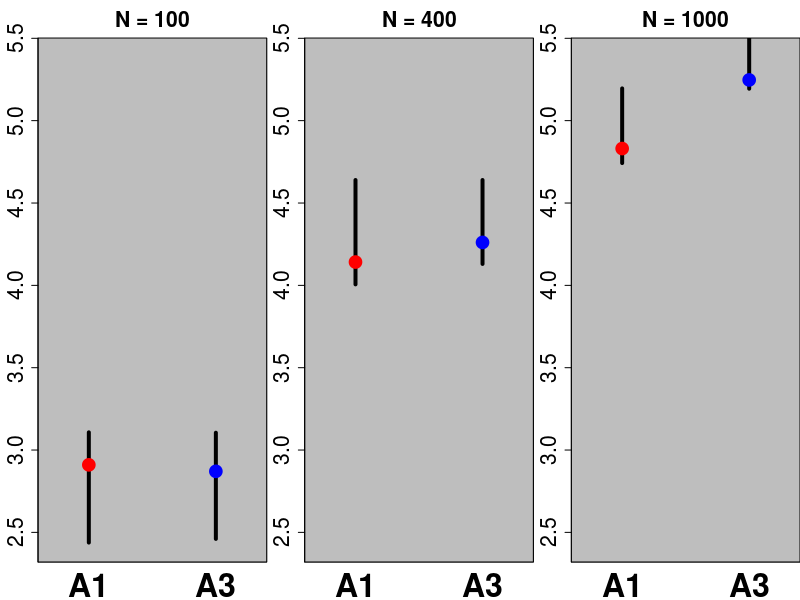
\includegraphics[width = 0.4\textwidth]{Times_Delta05}&
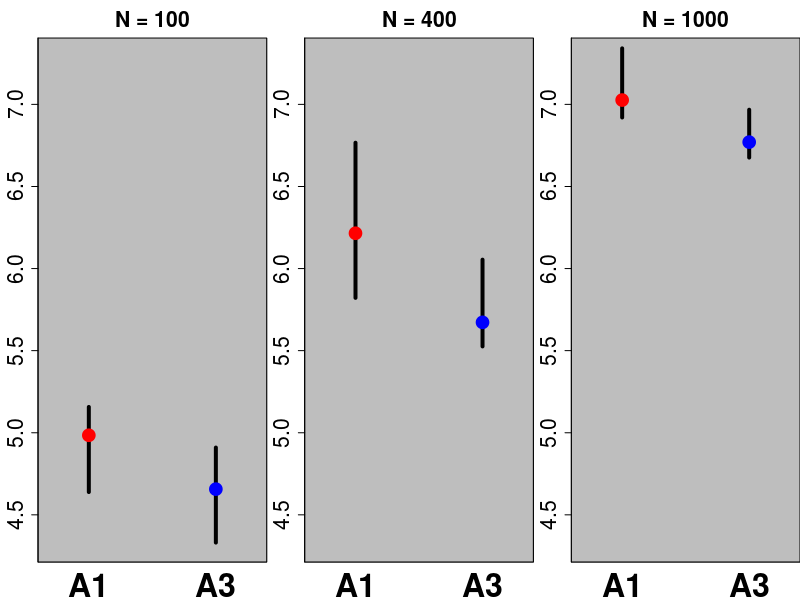
\includegraphics[width = 0.4\textwidth]{Times_Delta2}
\end{tabular}
\caption{Empirical distribution of required time (in logarithmic scale of milliseconds) for the acceptation of a candidate in the acceptance rejection algorithm of Lemma 1, depending on which bound is chosen. A1 is when the uniform bound is chosen, (see the paper), A3 is when the particle based bound is chosen. One can see that the best choice depends on the number of particles (as expected) but also on the time step. A3 gives the optimal bound, but a larger computationnal cost.}\label{Figure}
\end{figure}
This is now mentionned (without this empirical study) in the numerical experiments section (in the SINE model subsection).  We believe that it might be confusing to insist too much on this point by adding this study.

\item {\em Item 3 above should include a discussion regarding assumptions H1 and H2.}

\vspace{.3cm}

A few comments were added after these two assumptions.
Assumption H1 only involves the marginal likelihood $g_k$ of the observations and does not depend on our algorithm. In the case where the observations are given as in the practical section, this assumption holds as soon as the variance of the observation is bounded away from zero. Assumption H2 depends on the algorithm used to estimate the transition densities and on the tuning parameters of the  SMC filter. The most common choice is $\vartheta_k = 1$ so that under H1, the only requirement is to control $\widehat{q}_{k-1}$ and $p_{k-1}$. For instance, in the case of the GPE-1, as explained in Section~3, H2 is satisfied if $\phi$ is upper bounded (as for the EA1). 


\item {\em Can anything be said about the bias of the proposed estimator for finite $N$? Is it
only due to the form of  $\Lambda_k^N$ ?}

\vspace{.3cm}

The bias of forward backward based particle smoothers due to $\Lambda_k^N$ (i.e. to the particle approximations) was analyzed in \cite{delmoral:doucet:singh:2010}. In the case of additive functional as in (2), the bias of the forward only version of the FFBS algorithm is shown to be upper bounded by a term of order $n/N$ for strongly mixing hidden Markov models.  This bias is due to the form of  $\Lambda_k^N$ for the FFBS, FFBSi and PaRIS algorithms.


\item {\em What can be said about a CLT for the proposed estimator?}

\vspace{.3cm}

A CLT was derived for the original version of PaRIS algorithm as the number $N$ of particles grows to infinity. A CLT may also derived for our extension as it is a noisy version of the original method. However, even if its proof is not too involved it still require additional assumptions and technicalities. And the asymptotic variance remains hard to analyze (for instance to choose the parameters in comparison to other smoothing methods). Analyzing the variance of particle smoothers (FFBS, FFBSi, PaRIS, two-filer) is at the core of ongoing works and we believe that comparing the variance would be more suitable and interesting than just providing a CLT with no rules to choose between methods. We are also working on the estimation of such asymptotic variances which is a complex problem out of the scope of this paper.

\item {\em It is worth mentioning that, for the log-growth model, $X$ is a function of $\sigma$ and what
are the consequences of that in a context where $\sigma$ is an unknown parameter.}

\vspace{.3cm}

Even if there is no actual implementation of the EM algorithm in the paper for the log-growth model, we agree that providing some insights on the way it could be used may be very useful. We added a paragraph at the end of the log-growth section following the work of [4] explaining how the process can be transformed to estimate $\sigma$ using an EM algorithm although $X$ is a function of $\sigma$.

\item {\em I quite like the choice of $Q(\theta;\theta)$ in the examples. It would be very interesting to
have an implementation of the actual EM algorithm for parameter estimation in the
examples provided, using GRand Paris on the E step.}

\vspace{.3cm}

The numerical section now contains a complete implementation of a generalized EM algorithm for the SINE model which highlights clearly the performance of the proposed PaRIS algorithm.  
\end{enumerate}



\subsubsection*{Minor comments}
\begin{enumerate}
\item{\em page 3, line 36: The authors should clearly state that the proposed methodology
does not rely on time discretisation approximations.}

\vspace{.3cm}

This is now explicitly written in the introduction.

\item{\em page 5, line 21: computing $\longrightarrow$ computed.}

\vspace{.3cm}

This typo was corrected.

\item {\em page 8, line 52: I suggest "... $L_w$ is bounded below almost surely, ..."}

\vspace{.3cm}

This was changed as suggested.

\item {\em page 11, line 10: does the fixed lag algorithm have the same cost for all lag values?
What is the computational time of one run of GRand PaRIS for the examples presented?}

\vspace{.3cm}

The only cost difference for two lags $\delta_1 < \delta_2$ is the memory space to keep tracks of particles between times $t+\delta_1$ and $t+\delta_2$ (basically, a $N*(\delta_2 - \delta_1)$ matrix). Therefore the computationnal time is identical for two different lags.\\
On a personnal laptop  (i7-6600U CPU @ 2.60GHz), for the parameters given in the paper, it took around 25 seconds for each E step. As mentionned in the paper, all the comparisons are made for a same amount of computation time (that is why there is more particles used in the fixed lag techniques). 
This is now clarified in the paper.

\item {\em page 16, line 49: For the proof to be valid, the induction result needs to be established for $k\ge 0$.}

\vspace{.3cm}

\end{enumerate}

\bibliographystyle{plain}
\begin{thebibliography}{10}

\bibitem{delmoral:doucet:singh:2010}
P.~{D}el {M}oral, {A}.~{D}oucet, and {S}.{S}.~{S}ingh.
\newblock A backward particle intepretation of {F}eynman-{K}ac formulae.
\newblock {\em {ESAIM:~M2AN}}, 44:947--975, 2010.

\bibitem{olsson:westerborn:2016}
J.~Olsson and J.~Westerborn.
\newblock Efficient particle-based online smoothing in general hidden {M}arkov
  models: the {PaRIS} algorithm.
\newblock {\em ArXiv:1412.7550}, 2016.


\end{thebibliography}

\end{document}